\newcommand{\BaselineMeanVkt}{43.783}
\newcommand{\BaselineFactorTonnes}{16,791.5}
\newcommand{\BaselineCopertTonnes}{18,053.4}
\newcommand{\BaselineTerrainCoverage}{73.41}
\newcommand{\BaselineCommonCoverage}{99.996}
\newcommand{\SchedulingNetworkVktMean}{-0.0154}
\newcommand{\SchedulingNetworkVktMin}{-0.0155}
\newcommand{\SchedulingNetworkVktMax}{-0.0154}
\newcommand{\SchedulingParcelNetworkVktMean}{-9.48}
\newcommand{\SchedulingParcelNetworkVktMin}{-9.48}
\newcommand{\SchedulingParcelNetworkVktMax}{-9.48}
\newcommand{\SchedulingParcelVktMean}{-10.11}
\newcommand{\SchedulingParcelVktMin}{-10.11}
\newcommand{\SchedulingParcelVktMax}{-10.11}
\newcommand{\SchedulingFactorCoMean}{-0.0083}
\newcommand{\SchedulingFactorCoMin}{-0.0083}
\newcommand{\SchedulingFactorCoMax}{-0.0083}
\newcommand{\SchedulingCopertCoMean}{-0.0078}
\newcommand{\SchedulingCopertCoMin}{-0.0078}
\newcommand{\SchedulingCopertCoMax}{-0.0078}
\newcommand{\GradeNetworkVktMean}{-0.0237}
\newcommand{\GradeNetworkVktMin}{-0.0240}
\newcommand{\GradeNetworkVktMax}{-0.0232}
\newcommand{\GradeFactorCoMean}{+0.0033}
\newcommand{\GradeFactorCoMin}{+0.0023}
\newcommand{\GradeFactorCoMax}{+0.0046}
\newcommand{\GradeCopertCoMean}{-0.0153}
\newcommand{\GradeCopertCoMin}{-0.0156}
\newcommand{\GradeCopertCoMax}{-0.0150}
\newcommand{\GradeExposureMean}{-3.46}
\newcommand{\GradeExposureMin}{-3.47}
\newcommand{\GradeExposureMax}{-3.45}
\newcommand{\FactorFleetCoMean}{+7.52}
\newcommand{\FactorFleetCoMin}{+7.45}
\newcommand{\FactorFleetCoMax}{+7.60}
\newcommand{\DirectGradeCo}{+0.0063}
\newcommand{\GradeCoverageChange}{-0.130}

\subsection{Paired scheduling comparisons}
All five upstream realizations completed the 12-configuration design, yielding
30 assignments and 60 main emissions-configuration results, in addition to the
flat-grade diagnostic and fixed-source-trip control. Each scheduler serves
228,707 parcels with a maximum of 180 parcels on board. The inherited scheduler
produces 1,283 tours and the savings scheduler 1,332. Quantities by carrier and
customer zone are identical. More tours therefore coexist with lower travel
in this application; tour count alone does not describe scheduling efficiency.

At zero uphill penalty, parcel vehicle-kilometres change by
\SchedulingParcelNetworkVktMean\% over all network links, or
\SchedulingParcelVktMean\% on the common physical-road support.
Table~\ref{tab:scheduling} gives the corresponding common-support contrasts
at each path-cost coefficient. Parcel outcomes coincide to the displayed
precision across the five realizations: their spatial construction is
conditional on fixed demand, and supplied speeds do not vary by time.
The repeated values consequently do not supply five independent tests of
parcel scheduling effectiveness.

\begin{table}[htbp]
\centering
\caption{Savings scheduler relative to corrected inherited scheduling.
Paired percentage changes use common physical-road support; $u$ is the uphill
cost coefficient. Values are means; each parcel contrast coincides across realizations
at the shown precision.}
\label{tab:scheduling}
\begin{tabular}{@{}lrrr@{}}
\toprule Scheduling contrast (\%) & $u=0$ & $u=0.05$ & $u=0.20$ \\
\midrule
Parcel VKT & -10.11 & -10.12 & -10.17 \\
Parcel CO$_2$, inherited & -10.16 & -10.14 & -10.18 \\
Parcel CO$_2$, COPERT & -9.86 & -9.87 & -9.91 \\
\bottomrule
\end{tabular}

\end{table}

In the entire modelled network, the zero-penalty scheduling contrast changes
vehicle-kilometres by \SchedulingNetworkVktMean\% and common-support CO$_2$ by
\SchedulingFactorCoMean\% under inherited factors and
\SchedulingCopertCoMean\% under COPERT. Freight and service activity is held
fixed: the difference in whole-network totals is accounted for by the parcel
stream within numerical tolerance. The small aggregate percentages reflect
the parcel stream's share of this modelled activity, rather than an absence
of operational change within that stream.

\subsection{Terrain-informed path sensitivity}
With inherited parcel scheduling and the strongest tested uphill coefficient
($u=0.20$), network VKT changes by \GradeNetworkVktMean\%
(replicate range \GradeNetworkVktMin\% to \GradeNetworkVktMax\%).
Absolute-grade-weighted physical-road travel changes by \GradeExposureMean\%.
Common-support CO$_2$ changes by \GradeFactorCoMean\% under inherited factors
(range \GradeFactorCoMin\% to \GradeFactorCoMax\%), compared with
\GradeCopertCoMean\% under COPERT
(range \GradeCopertCoMin\% to \GradeCopertCoMax\%).
Thus, the mean CO$_2$ response differs in sign between configurations despite
the reduction in VKT. Figure~\ref{fig:grade} displays the cost sensitivity.
The result concerns the specified route preferences and factor/fleet assumptions;
Dijkstra's selected objective is not CO$_2$ minimization.

\begin{figure}[htbp]
\centering
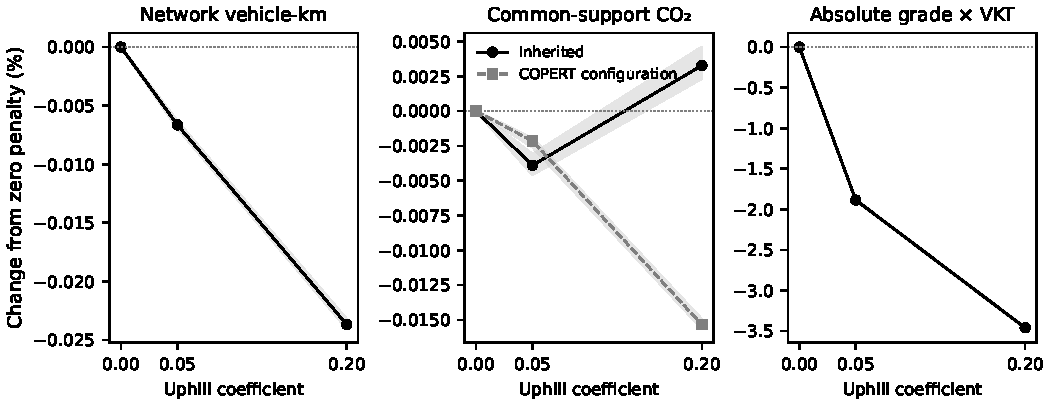
\includegraphics[width=\linewidth]{../results/dutch-pilot/grade-effects.pdf}
\caption{Grade-cost sensitivity with inherited parcel scheduling. Lines are
means and shading spans the minimum and maximum over five paired upstream
realizations, not confidence intervals. The coefficient has case cost units
per kilometre per percentage point of uphill grade. VKT includes all network
links; CO$_2$ uses common physical-road factor support; grade-weighted travel
uses physical links and flagged zero fallbacks.}
\label{fig:grade}
\end{figure}

At zero penalty, retained terrain proxies cover \BaselineTerrainCoverage\%
of physical-road VKT on average. This share changes by
\GradeCoverageChange\ percentage points at $u=0.20$ with inherited scheduling.
Because fallback links carry zero assumed grade, path changes can favour
unsampled or screened links. Lower modelled grade exposure therefore cannot
be interpreted directly as verified avoidance of real road slopes.

\subsection{Emissions configuration on fixed activity}
At zero uphill penalty with inherited scheduling, mean common-support CO$_2$
is \BaselineFactorTonnes\,t under inherited factors and
\BaselineCopertTonnes\,t under COPERT: a paired mean change of
\FactorFleetCoMean\% (range \FactorFleetCoMin\% to \FactorFleetCoMax\%).
The common support covers \BaselineCommonCoverage\% of physical-road VKT.
These totals compare the supplied factor/fleet configurations; the modern
COPERT fleet is not matched to the inherited factors' fleet assumptions.
Fuel-carbon conventions also remain those of each configuration, so their
difference cannot be assigned to the emissions formula alone.

On the same zero-penalty activity, introducing the terrain proxy into COPERT
factors changes common-support CO$_2$ by \DirectGradeCo\% on average, without
any path change. This direct response is distinct from the route-cost contrasts
above. The supplied van coefficients are grade-insensitive, so the parcel
stream has no corresponding direct grade-factor response. The experiments
therefore separate scheduling, path selection and emissions accounting while
retaining the limits imposed by the current data and coefficient tables.
